\documentclass[a4paper,12pt]{scrartcl}

\author{Matthew Cocci}
\title{Title}
\date{today}
\usepackage{enumitem} %Has to do with enumeration	
\usepackage{amsfonts}
\usepackage{amsmath}
\usepackage{amsthm} %allows for labeling of theorems
\usepackage[T1]{fontenc}
\usepackage[utf8]{inputenc}
\usepackage{blindtext}
\usepackage{graphicx}
%\numberwithin{equation}{section} 
%, This labels the equations in relation to the sections rather than other equations
%\numberwithin{equation}{subsection} %This labels relative to subsections
\newtheorem{thm}{Theorem}[section]
\newtheorem{lem}[thm]{Lemma}
\newtheorem{prop}[thm]{Proposition}
\newtheorem{cor}[thm]{Corollary}
\setkomafont{disposition}{\normalfont\bfseries}
\usepackage{appendix}


\begin{document}

\begin{center} \LARGE \bf
   The Multivariate Normal Distribution
\end{center}

The univariate normal distribution is an extremely familiar concept
where some random variable $X$ can take values along the real with 
probabilities that match the famouse bell-curve. Recall 
the probability density function of
   \[ f_Y(y) = \frac{1}{\sigma \sqrt{2\pi}} \; e^{-\frac{1}{2\sigma^2}
      (y - \mu)^2} \]
However, that's 
limited to only one dimension, and we would like to generalize to 
higher dimensions. In the next-simplest
2-dimensional case, we'd like a distribution
that actually looks like a bell---where potentional values can
range over the real plane, $\mathbb{R}$, where the density is
clustered around some mean before tapering off in all directions, 
as seen below.
\begin{figure}[h!]
   \centering
   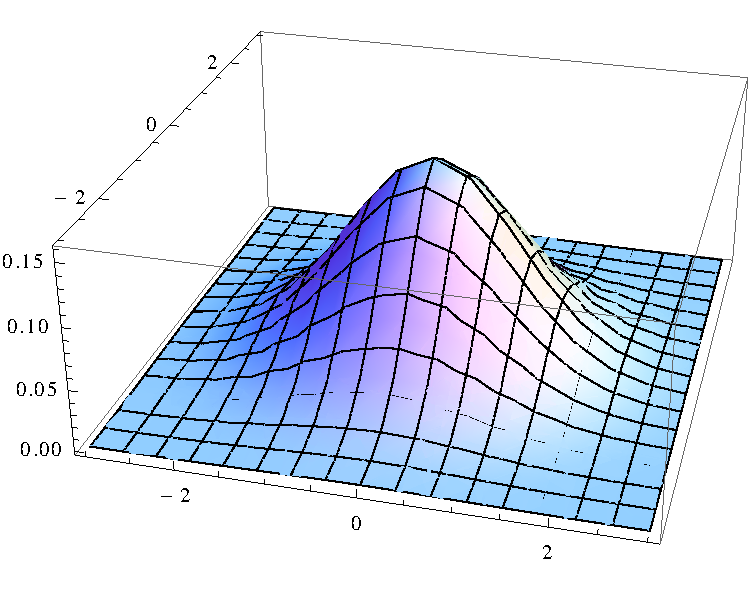
\includegraphics[scale=0.40]{multivariate.pdf}
\end{figure}
\\
This figure has mean zero for both $X_1$ and and $X_2$, and 
which are independent, implying $\sigma = I_2$, the identity matrix. 
It's easy to see that any vertical cuts parallel to $xz$ or $yz$ planes
will yield a traditional normal random variable. This of course 
generalizes to higher dimensions, although we can't display it so nicely.

\section{Notation}

In this note, the multivariate distribution will apply to a
$d$-dimensional random vector 
\[ \mathbf{X} = \begin{pmatrix} X_1 & X_2 & \ldots & X_d \end{pmatrix}^T,
    \qquad \mathbf{X}  \sim N_d(\mu, \Sigma) \]
where $\mu$ is the $n$-dimensional \emph{mean vector},
\[ \mu = \begin{pmatrix} EX_1 & EX_2 & \ldots & EX_d \end{pmatrix}^T,
      \]
and where $\Sigma$ is the $d\times d$ \emph{covariance matrix}, which
is defined and has in its $i,j$ entry
\[ \sigma^2 = E\left[ (\mathbf{X} - \mu) (\mathbf{X}-\mu)^T\right] \in
   \mathbb{R}^{N\times N} \] 
\[ \Sigma_{ij} = Cov(X_i, X_j), \qquad i,j = 1, \ldots, d\]
All MVN random variables (and random vectors, more generally) will be in 
boldface, such as $\mathbf{X}$ for easy subscripting.  
$\mathbf{X}_t$ will indicate the random vector $\mathbf{X}$ at 
time $t$, while $X_i$ indicates the $i$th element of $\mathbf{X}$.
Constants, vectors of constants, and matrices of constants will not be 
in boldface.

\newpage

\section{Definition}

A random vector $\mathbf{X}$ has a \emph{multivariate normal} 
distribution if every linear combination of its components,
\[ Y = a_1 X_1 + \ldots + a_d X_d \] 
\[ \Leftrightarrow Y = {a} \mathbf{X}, \qquad
    {a} \in \mathbb{R}^{d} \]
is \emph{univariate normally
distributed}, with a corresponding mean and variance. This gives a 
joint density function of 
\begin{equation}
    \label{pdf}
   f_{X}({x}) = \frac{1}{(2\pi)^{d/2}\lvert \Sigma \rvert^{1/2}} 
	\; e^{ -\frac{1}{2} ({x} - \mu)^T \;
	\Sigma^{-1} ({x} - \mu) }, \qquad \lvert\Sigma\rvert =
      \det\Sigma \qquad x \in \mathbb{R}^d
\end{equation}
Note, we impose the requirement that $\Sigma$ is symmetric and positive 
definite.  Symmetric because the correlation of $X$ and $Y$ equals the
correlation of $Y$ and $X$. 
\\
\\
{\sl Terminology}: I'll often us MVN to refer to the case where $\mathbf{X}$ is
a vector with $d\geq2$; however, it should be clear that the univariate
normal distribution is just a special case where $d=1$. Therefore,
when speaking about an RV that could be either MVN or univariate normal
\emph{or} properties that apply equally well to either
type of RV, I'll often use the term \emph{Gaussian}
both for convenience and out of reverence to long-dead German-speaking
mathematicians. Stimmt?


\section{Linear Transformations of MVN Random Variables}

It's fairly common to consider linear transformations and functions
of a multivariate normally distributed random variable.  For instance,
we might have an economic or statistical model with a recurrence 
relation to describe the dynamics of some process:
\[ \mathbf{X}_{t+1} = A \mathbf{X}_{t} + \mathbf{V}_{t+1} \]
where $\mathbf{V}_t$ is some innovation or random noise vector.
Therefore, it would be useful to be able to derive the distributions
of \emph{functions} or \emph{linear transformation} of multivariate 
normal random variables.

\subsection{Transformation Theory Recap}

So let $\mathbf{X} = A\mathbf{Y}$. Suppose we have the distribution of
$\mathbf{X}$, denoted $f_{{X}}$, and we want the distribution
of $\mathbf{Y}$, $f_{{Y}}$. Then
\begin{align}
    f_{{Y}}(y) &= |\det(A)| \; f_{{X}}(Ay) \notag \\
    f_{{X}}(x) &= \frac{1}{|\det(A)|} \; f_{{Y}}(A^{-1} x) 
	\label{trans}
\end{align}

\newpage
\subsection{Derivation of Probability Distribution}

So let's find the probability distribution of a linear transforamtion
of an MVN RV. Begin by assuming 
\begin{align*}
    \mathbf{X} &= A\mathbf{Y}, \qquad \mathbf{Y} \sim 
	\text{MVN}(\mu, \Sigma) \\
    \Rightarrow \quad f(y) &= k \; \exp\left\{-\frac{1}{2} (y - \mu)^T 
	\; \Sigma^{-1} (y-\mu)\right\}
\end{align*}
where $k$ is a constant.\footnote{The constant will come from the
definition of the distribution given above in Equation \ref{pdf}, but
it's boring algebra not that interesting, so I'll suppress the details.}
Assuming that $A$ is invertible, we substitute in, using Equation 
\ref{trans}, to get the distribution of $\mathbf{X}$:
\begin{align}
    \label{midway}
    \Rightarrow \quad f_X(A^{-1}x) &= k' \exp\left\{-\frac{1}{2} (A^{-1}x - \mu)^T 
	\Sigma^{-1} (A^{-1}x-\mu)\right\} 
\end{align}
Next, since the expectation is a linear operator, we can use the fact
that 
\begin{align*}
    E\mathbf{X} &= E[A\mathbf{Y}] = A E\mathbf{Y} = A \mu \\
    \Rightarrow \quad \mu_* &= A \mu \\
    \Leftrightarrow \quad \mu &= A^{-1} \mu_*
\end{align*}
where $\mu'$ is the mean vector of $\mathbf{X}$.  With that, we
can substitute back into Equation \ref{midway} and simplify even
further, using convenient matrix manipulations like the distributivity
property, associativity, etc.:
\begin{align*}
    f_X(A^{-1}x) &= k' \exp\left\{-\frac{1}{2} (A^{-1}x - \mu)^T \;
	\Sigma^{-1} (A^{-1}x-\mu)\right\} \\
    &= k' \exp\left\{-\frac{1}{2} (A^{-1}x - A^{-1}\mu_*)^T \;
	\Sigma^{-1} (A^{-1}x-A^{-1}\mu_*)\right\} \\
    &= k' \exp\left\{-\frac{1}{2} [A^{-1}(x - \mu_*)]^T \;
	\Sigma^{-1} [A^{-1}(x-\mu_*)]\right\} \\
    &= k' \exp\left\{-\frac{1}{2} (x - \mu_*)^T \; [(A^{-1})^T \;
	\Sigma^{-1} A^{-1}] (x-\mu_*)\right\} \\
    &= k' \exp\left\{-\frac{1}{2} (x - \mu_*)^T \;  
	\Sigma_*^{-1} \; (x-\mu_*)\right\} \\
    \Rightarrow \mathbf{X} &\sim  \text{MVN}(\mu_*, \Sigma_*), 
    \qquad \text{where $\mu_* = A\mu$ and $\Sigma_* = A\Sigma A^T $}
\end{align*}
This is huge! It means \emph{linear transformations of MVN
RV's are themselves MVN.}


\newpage
\section{From Standard to General MVN Random Variables}

If you're familiar with the standard univariate normal RV,
then you can probably guess what the standard MVN RV is:
\begin{equation}
    \mathbf{Z} \sim \text{MVN}(0, \; I_d) 
\end{equation}
where $I_d$ is the $d\times d$ identity matrix.  This form for
the covariance matrix also suggests that the different components
of $\mathbf{Z}$ (denoted $Z_1, Z_2, \ldots, Z_d$) are independent and
Gaussian.
\\
\\
Moreover, just like we can build from a standard univariate to
a general univariate.  To do so, we'll use the results from the 
last section, since building from a standard MVN
to general MVN simply involves linear transformations of the components.
Specifically, we can express the MVN RV $\mathbf{X}$ as follows
\begin{equation}
    \mathbf{X} = \mu + A\mathbf{Z}, \qquad \mathbf{X}\sim 
	\text{MVN}(\mu, AA^T)
\end{equation}
{\sl Computation}: Suppose we know that we want $\mathbf{X}$ to
be MVN($\mu, \; \Sigma)$, and we can only generate $\mathbf{Z}$.
How do we choose $A$ such that $AA^T = \Sigma$.  Typically, we'll
have to use something like a \emph{Cholesky Factorization}
algorithm to find the correct $A$ in the form of a lower triangular
matrix. And if $\Sigma$ is symmetric, positive definite, then 
$A$ is guaranteed to exist and this approach will work. 
The algorithm itself can be found in the appendix.


\section{Facts About Multivariate Normal Random Variables}

So to summarize, MVN (or Gaussian) RV's are particularly nice to work with because
of some convenient properties:
\begin{enumerate}
    \item Suppose that $\mathbf{X}$ and $\mathbf{Y}$ are \emph{univariate}
	normally distributed and independent. This then implies that they are 
	\emph{jointly normally distributed}. In other words, 
	$\begin{pmatrix} \mathbf{X} & \mathbf{Y} \end{pmatrix}$ must have a multivariate
	normal distribution. 
    \item Linear functions of Gaussians are Gaussian. So if $A$
	is a constant matrix and $\mathbf{X}$ is MVN, then $A\mathbf{X}$
	is also MVN.
    \item Uncorrelated Gaussian random variables are independent.
    \item Conditions Gaussian's are normal. So if $X_1$ and $X_2$
	are two components of a MVN RV, $\mathbf{X}$, then 
	$X_1 | X_2$ is normal, and vice versa.
\end{enumerate}






\end{document}

